\chapter{User Interface Specification}

% This section contains mockups, descriptions,
% and explanations, lots of graphics
\section{Preliminary Design}

\subsection{Company}
From this page, you are able to view details statistics about certain companies after being linked to it or searching for it. Major details, such as the quote, are up at the top while further details are at the bottom. A user can comment on the company on the bottom right. If you decide that you want to trade, you simply press the trade button and a box will pop-up, giving you options for the trade.//
\begin{figure}
\centering
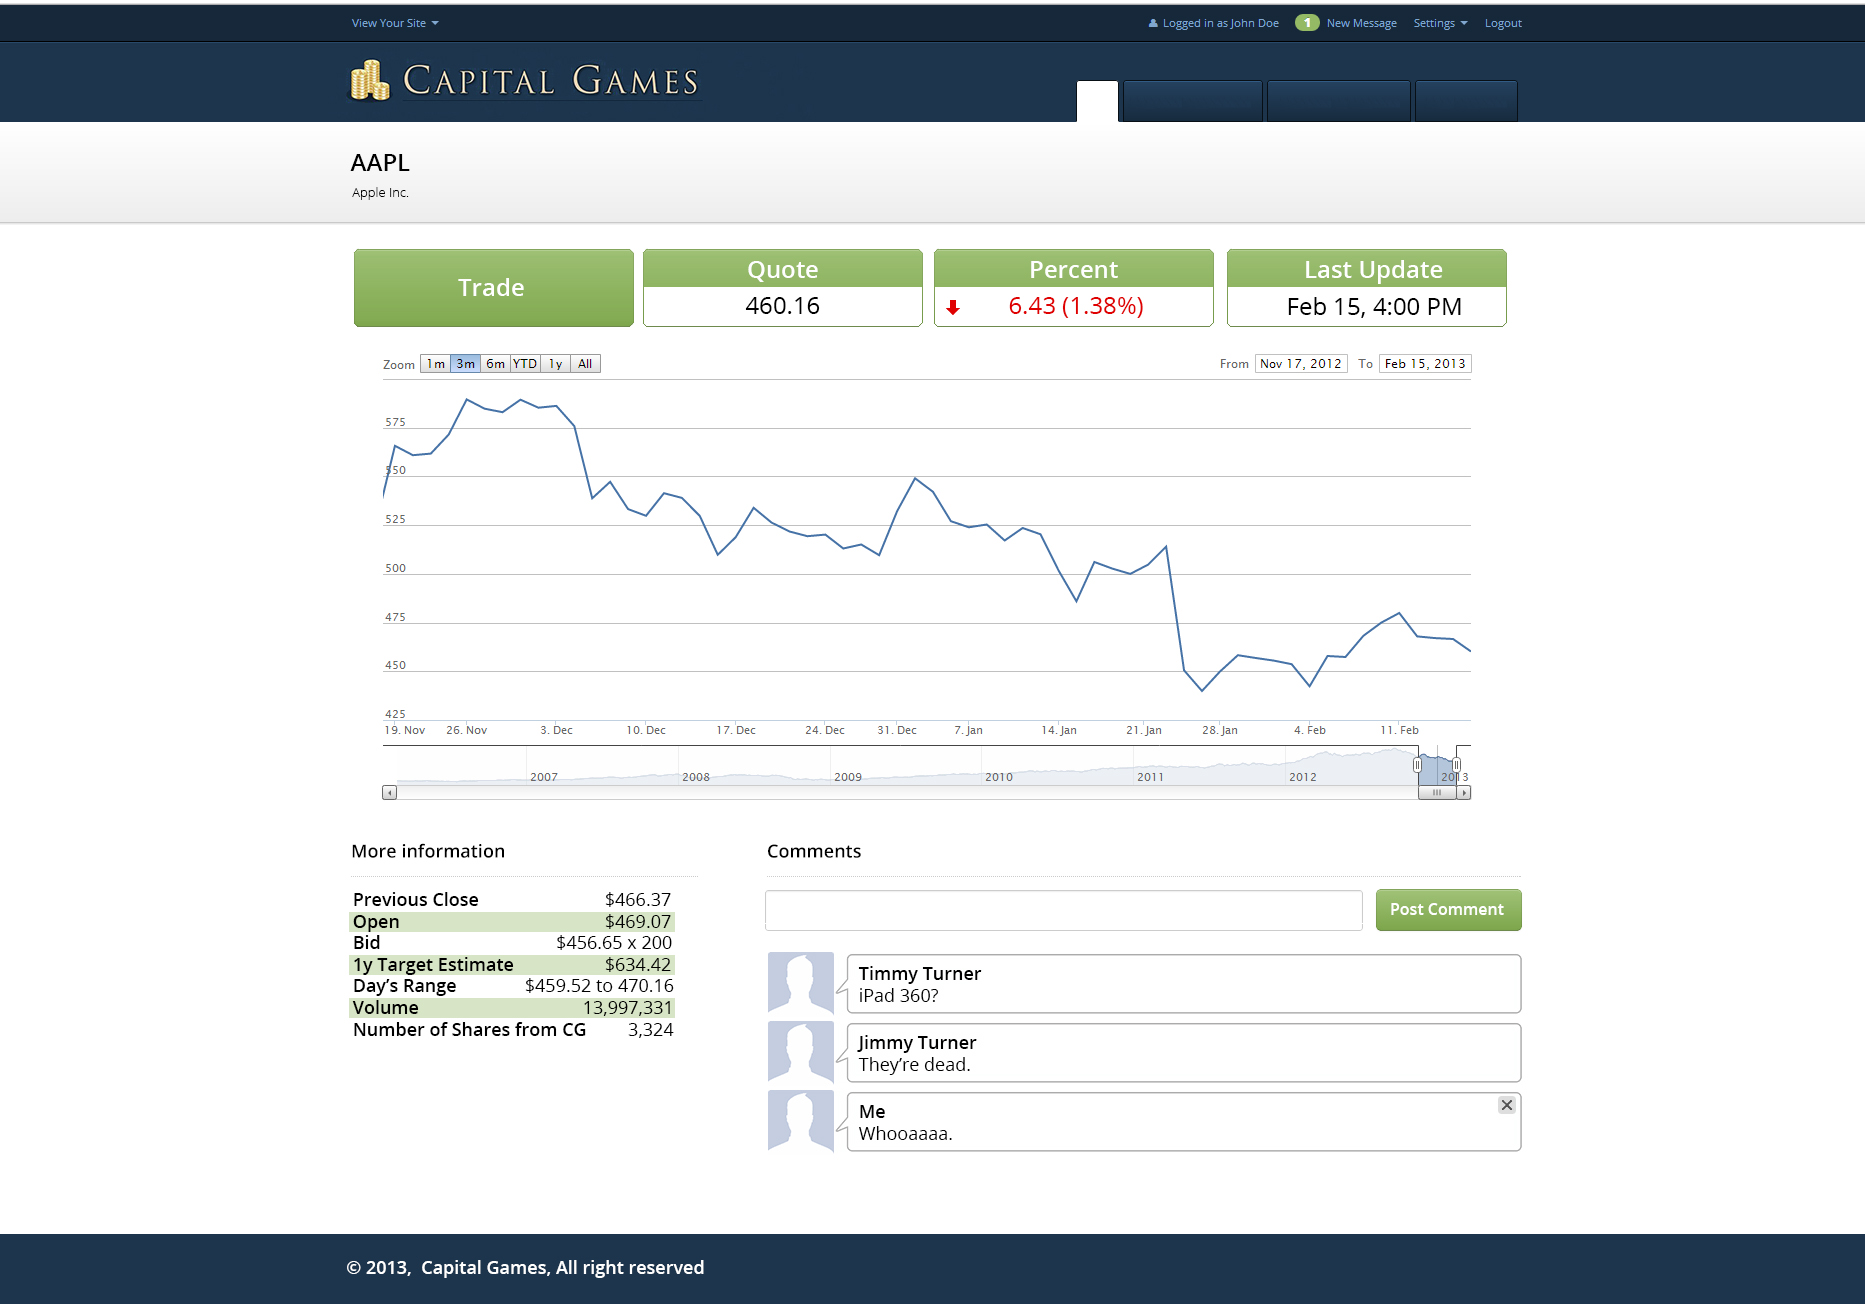
\includegraphics[width=5.5in]{./mockups/JPEG/company.jpg}
\end{figure}
\begin{figure}
\centering
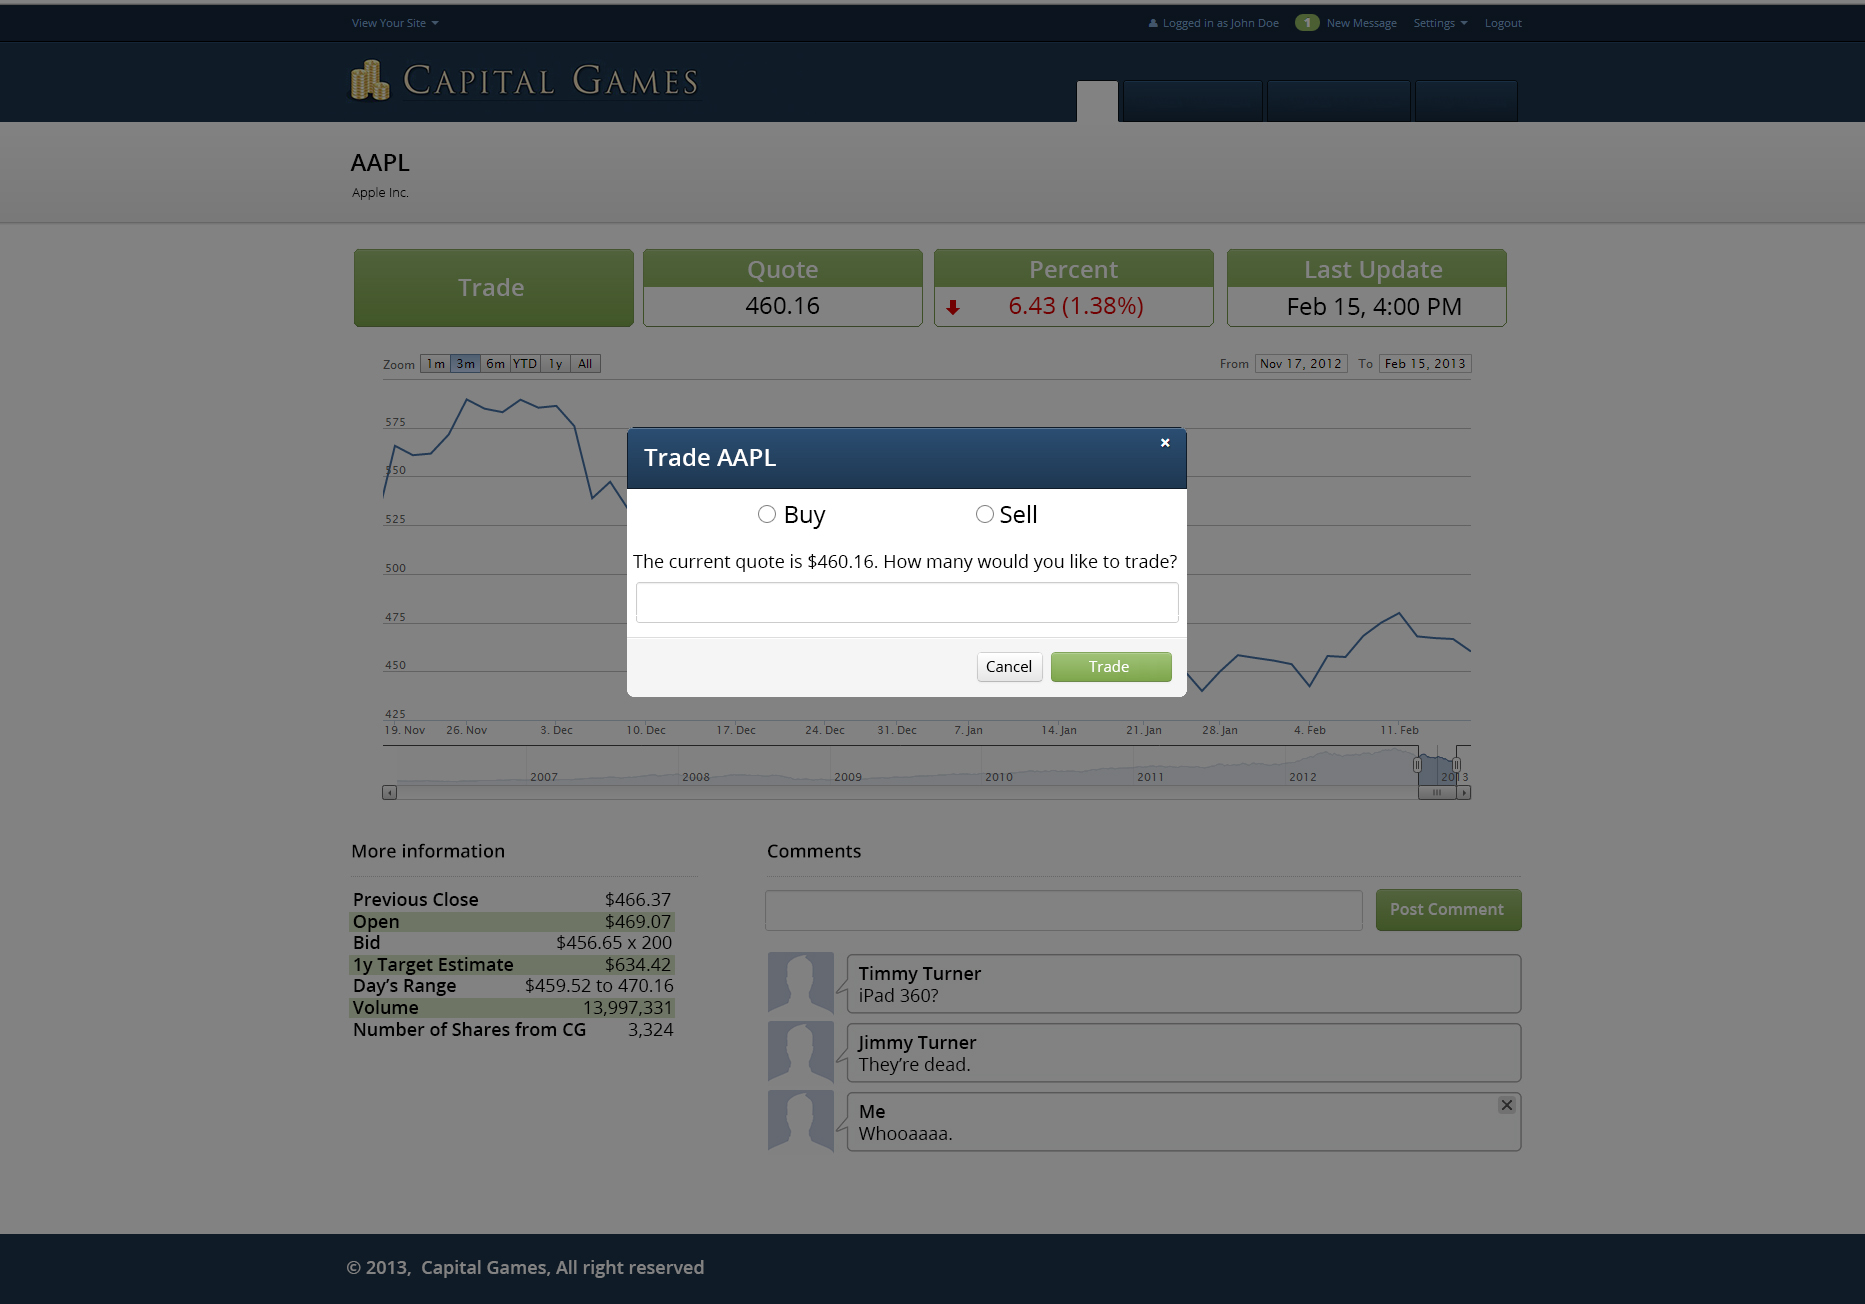
\includegraphics[width=5.5in]{./mockups/JPEG/Trade_popup.jpg}
\end{figure}

\subsection{League}
From this page, you are able to view a certain league. Up at the top are the main facts about the league as well as a button to join/quit the league and the icon for it. In the middle, there is a ranking system to show the users in the highest standing. Down at the bottom, you can see the activity and also comment on the league itself. //
\begin{figure}
\centering
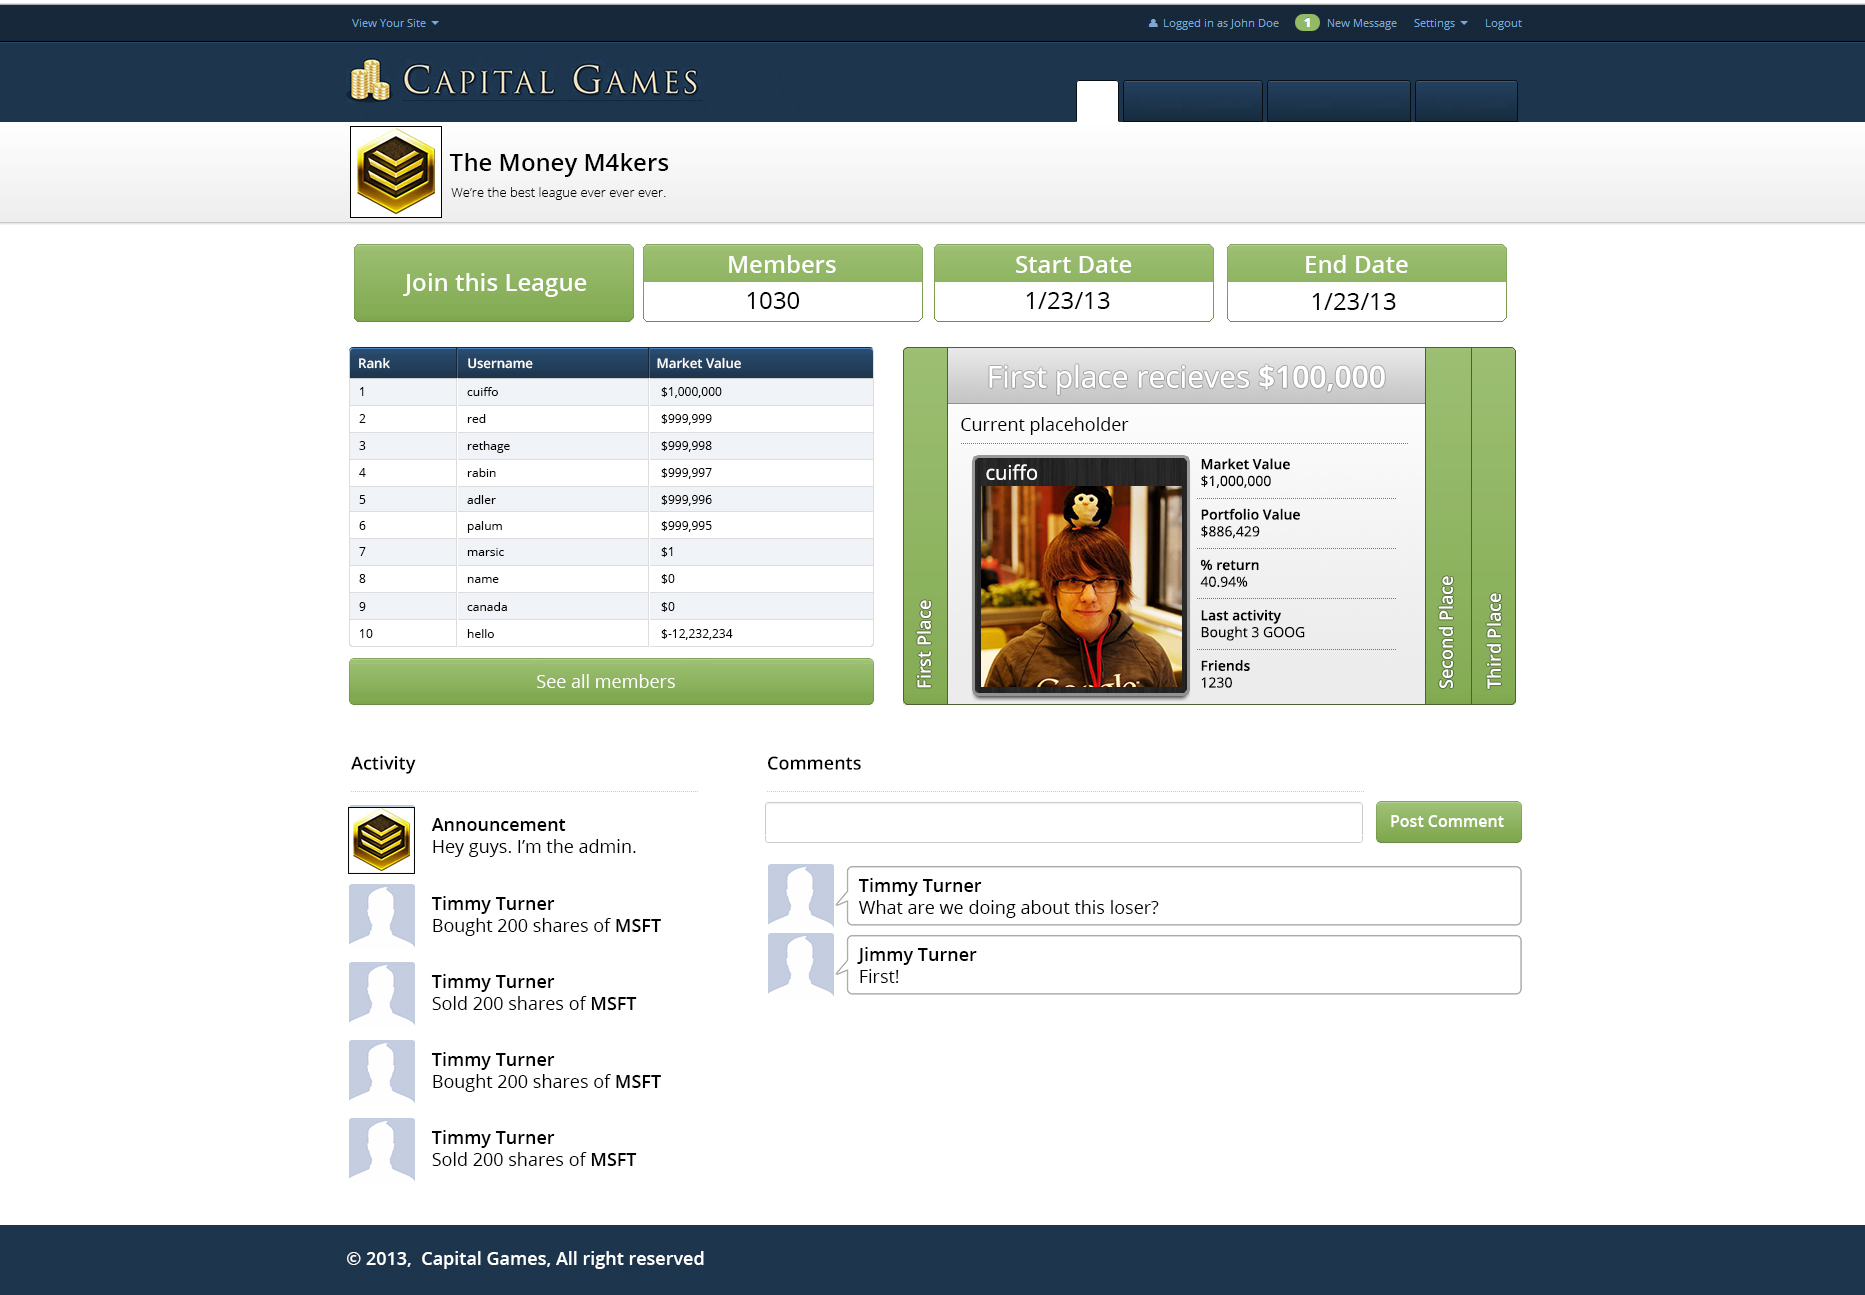
\includegraphics[width=5.5in]{./mockups/JPEG/Leagues_third.jpg}
\end{figure}

\subsection{League Admin}
A league admin will see the join/quit button on a league as the settings page for them. When they click on that, they are brought to a page that gives them many settings they can change for the league, the most typical being the name, description and icon.//
\begin{figure}
\centering
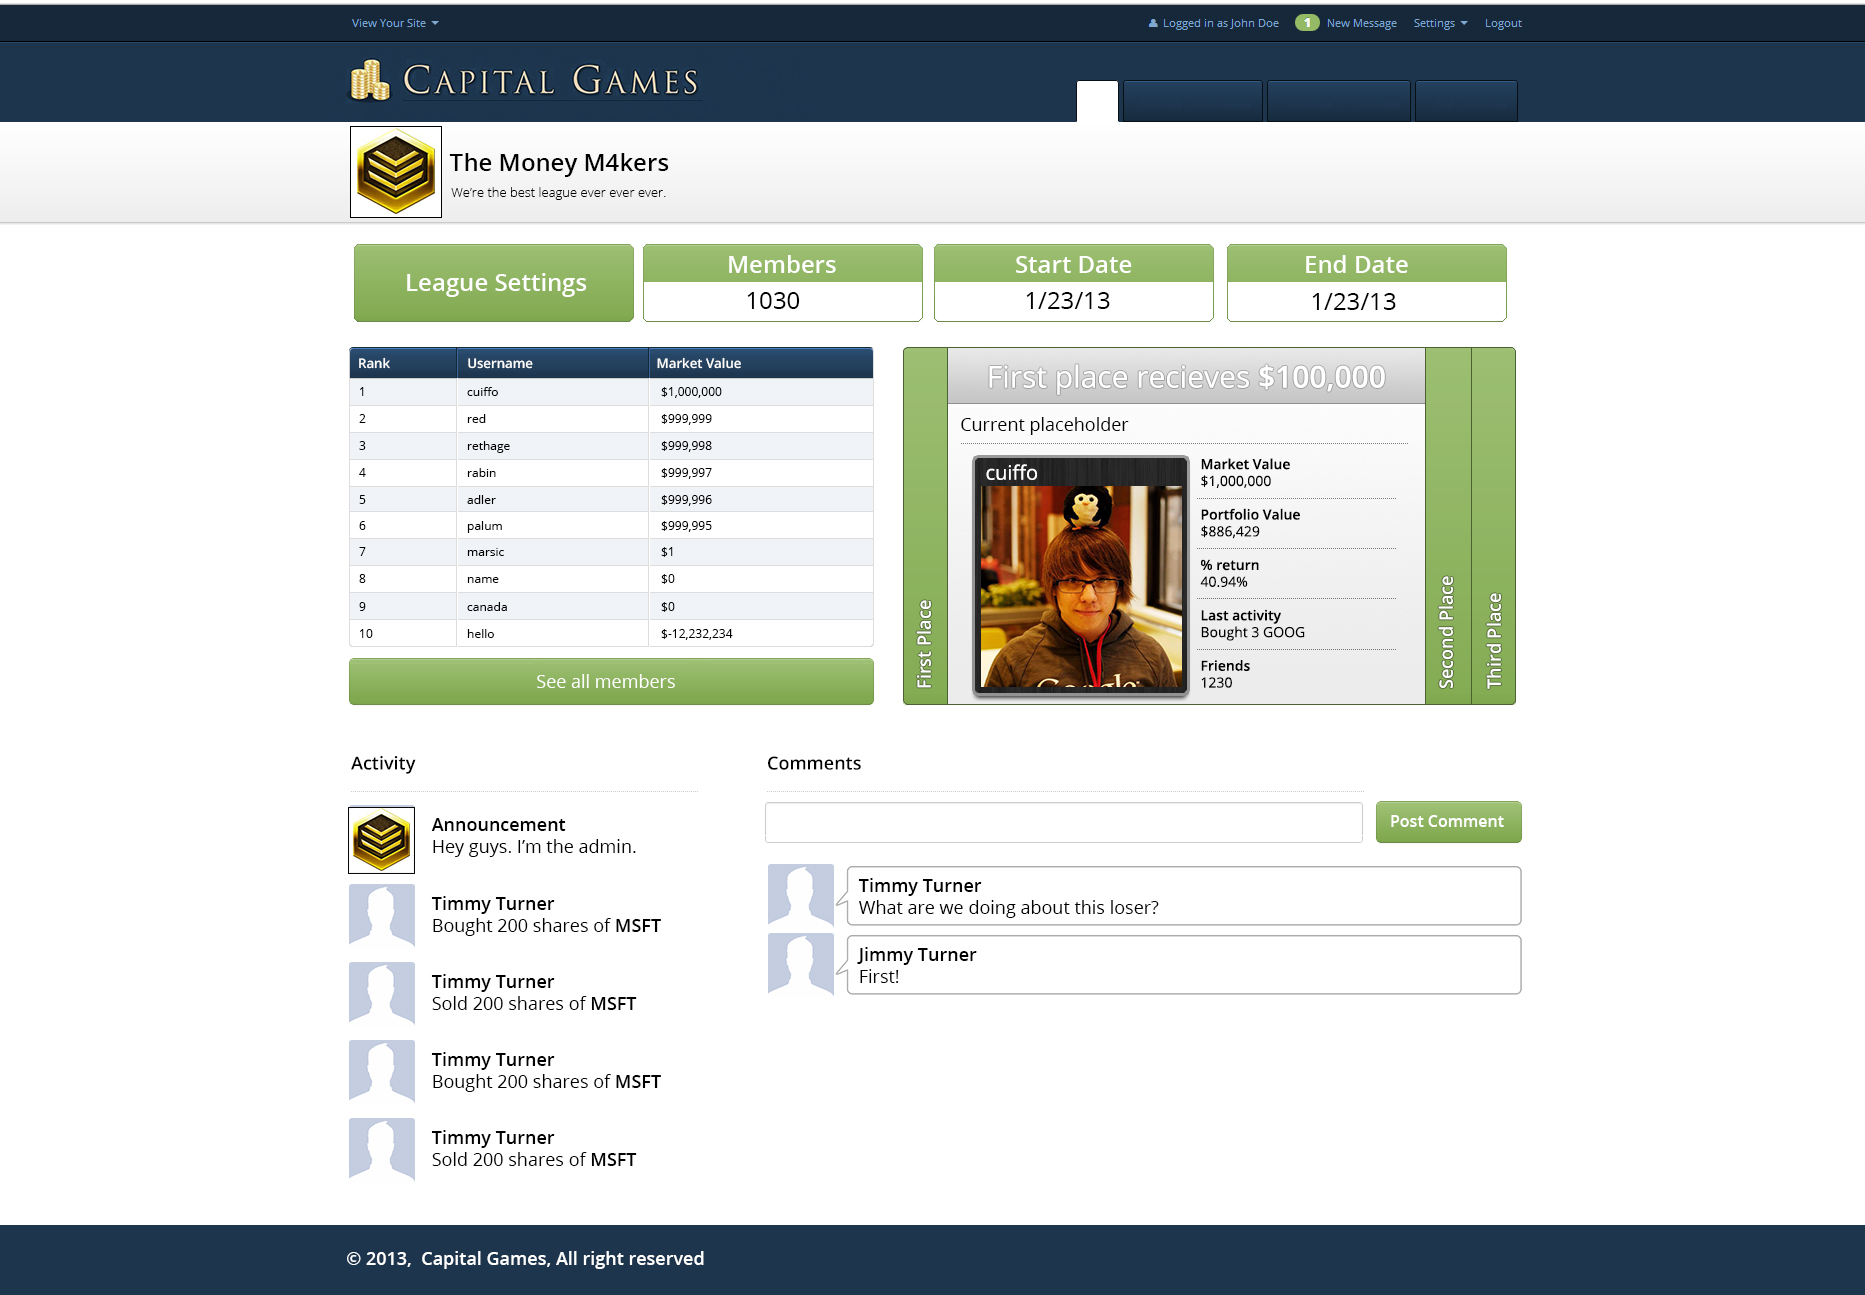
\includegraphics[width=5.5in]{./mockups/JPEG/Leagues_admin.jpg}
\end{figure}
\begin{figure}
\centering
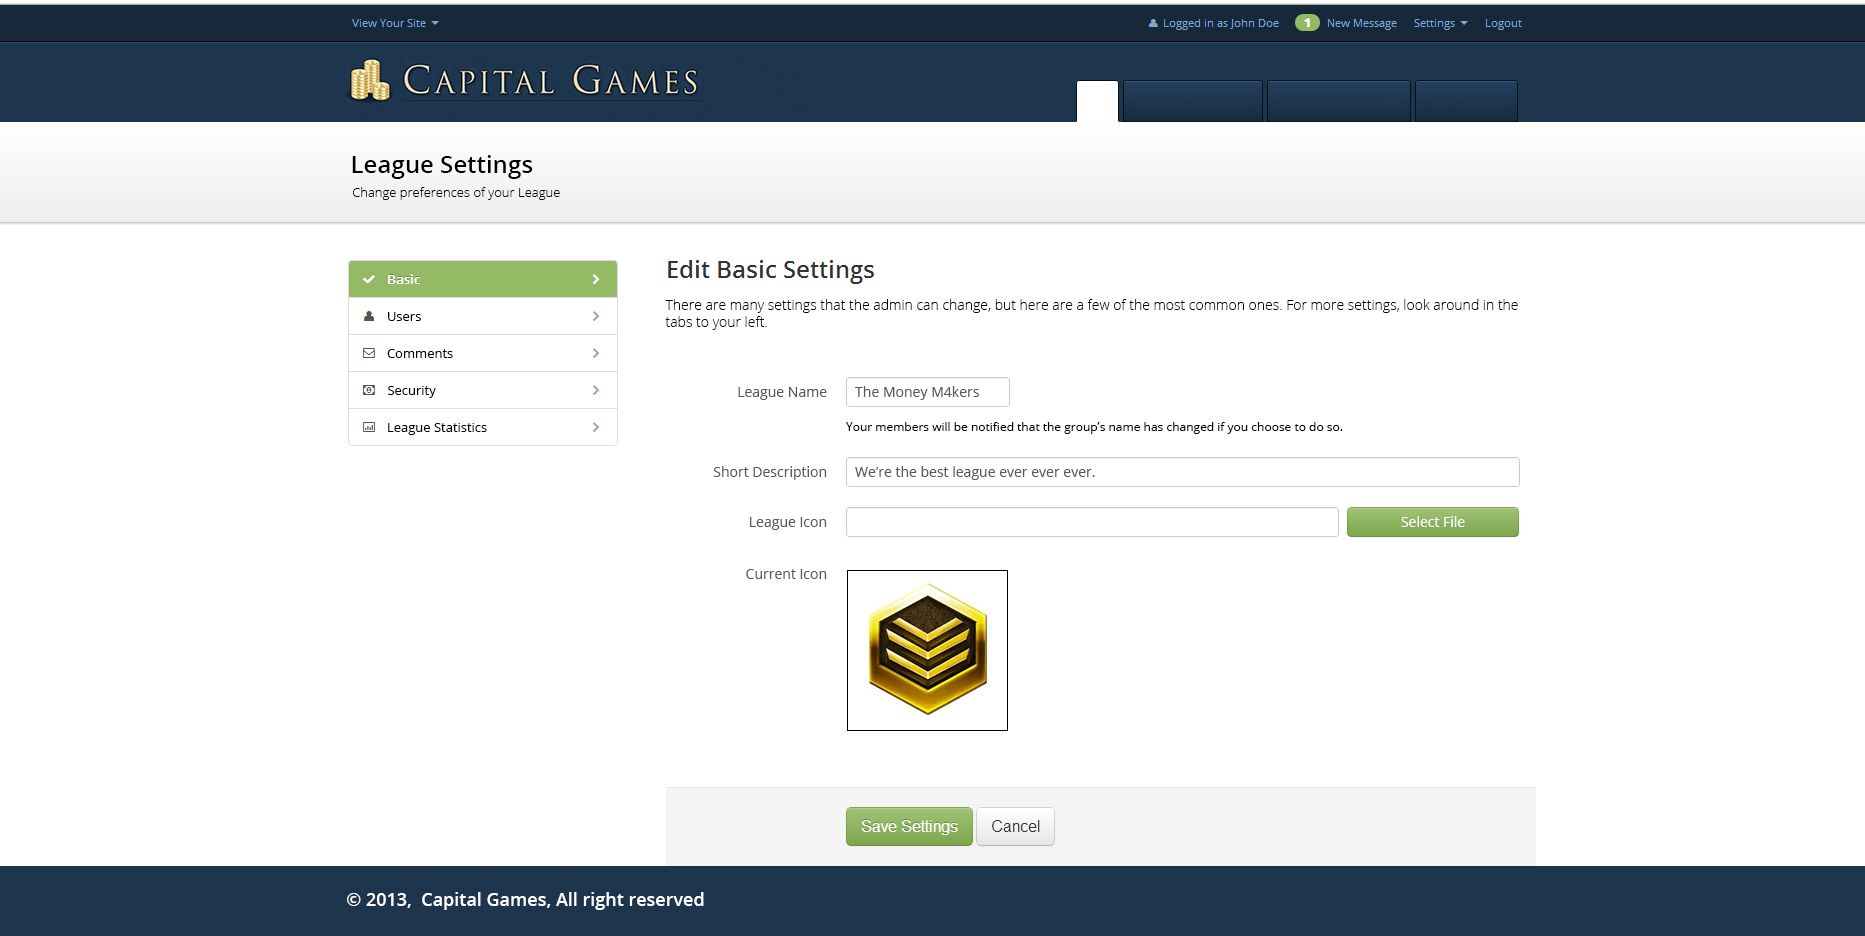
\includegraphics[width=5.5in]{./mockups/JPEG/league_admin.jpg}
\end{figure}


\subsection{Messages}
A league admin will see the join/quit button on a league as the settings page for them. When they click on that, they are brought to a page that gives them many settings they can change for the league, the most typical being the name, description and icon.//
\begin{figure}
\centering
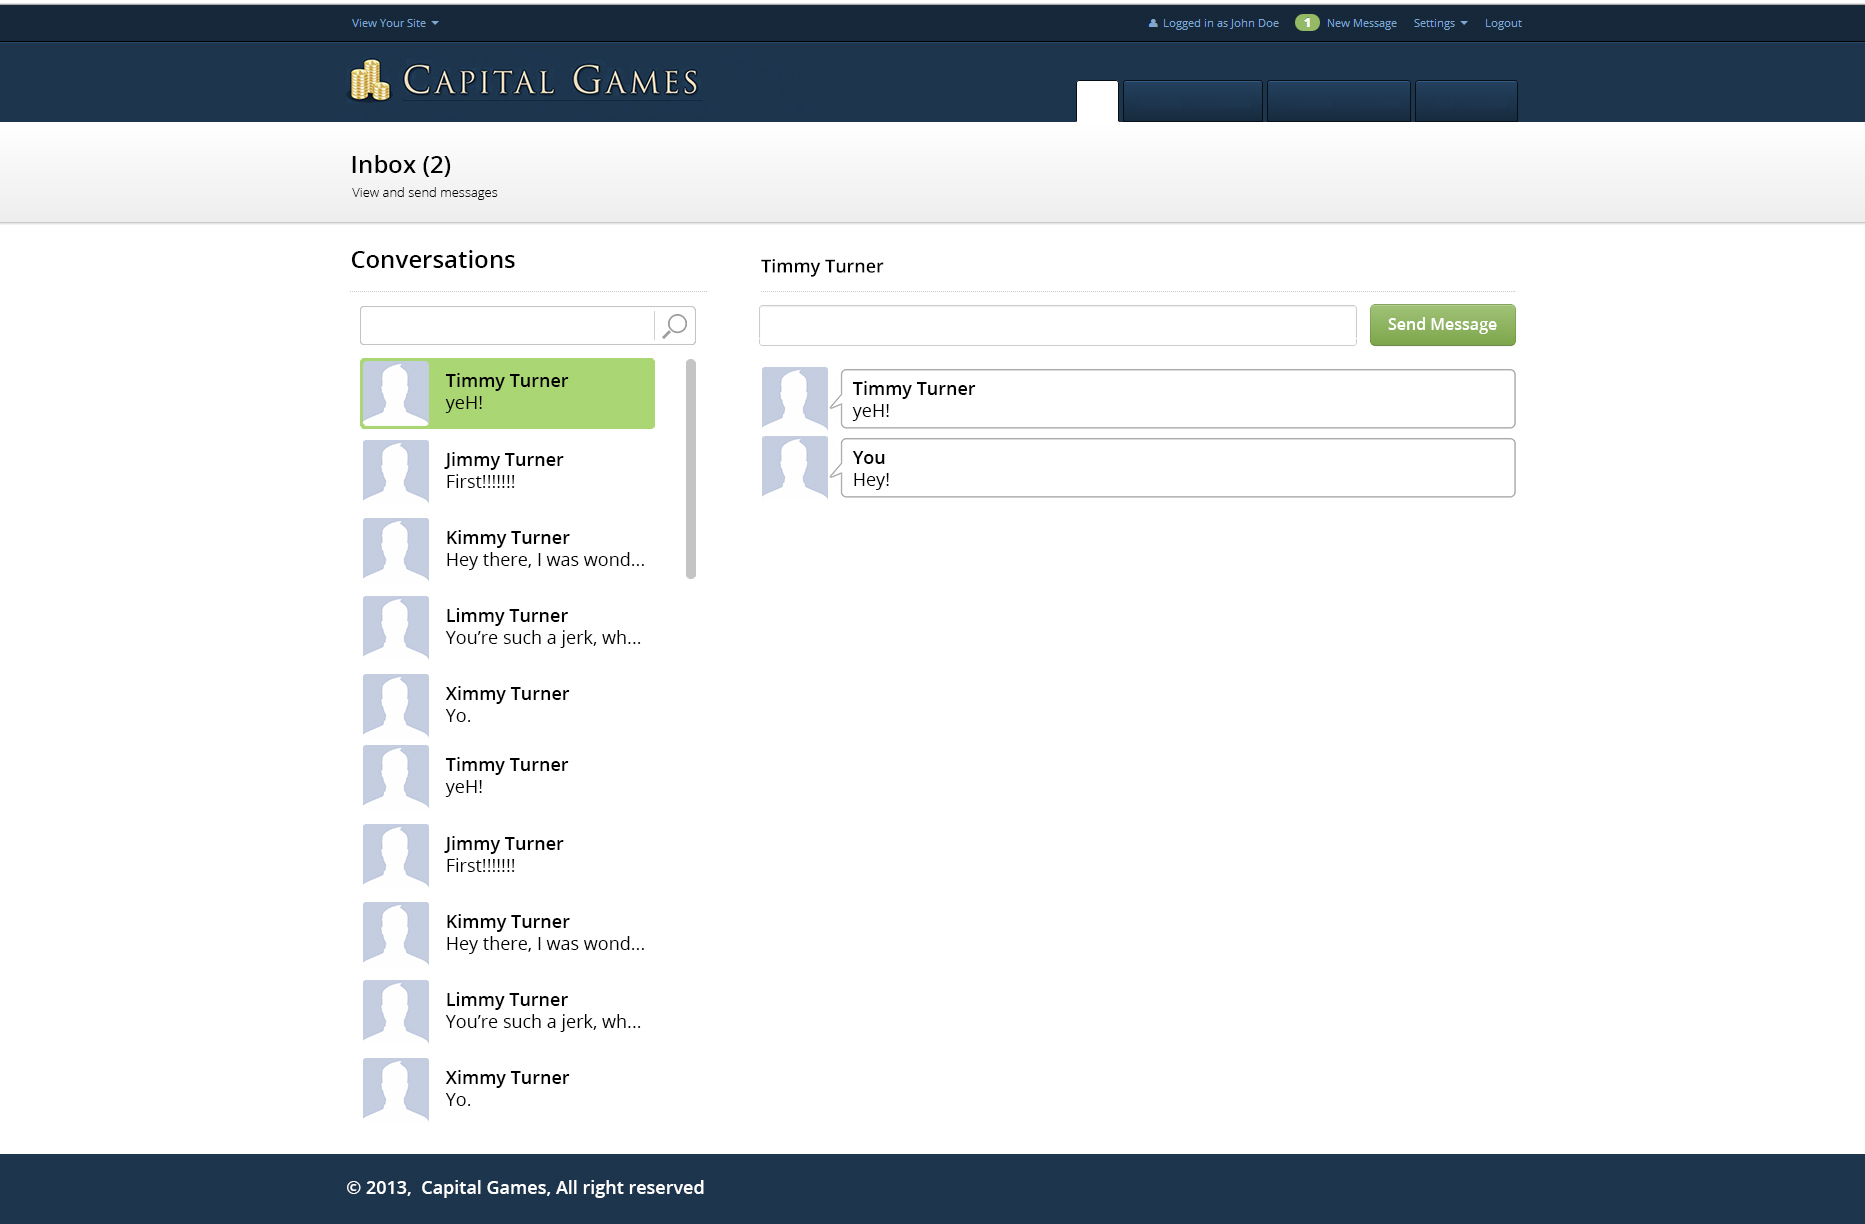
\includegraphics[width=5.5in]{./mockups/JPEG/messages.jpg}
\end{figure}
\subsection{Login}
{
\begin{figure}
\centering
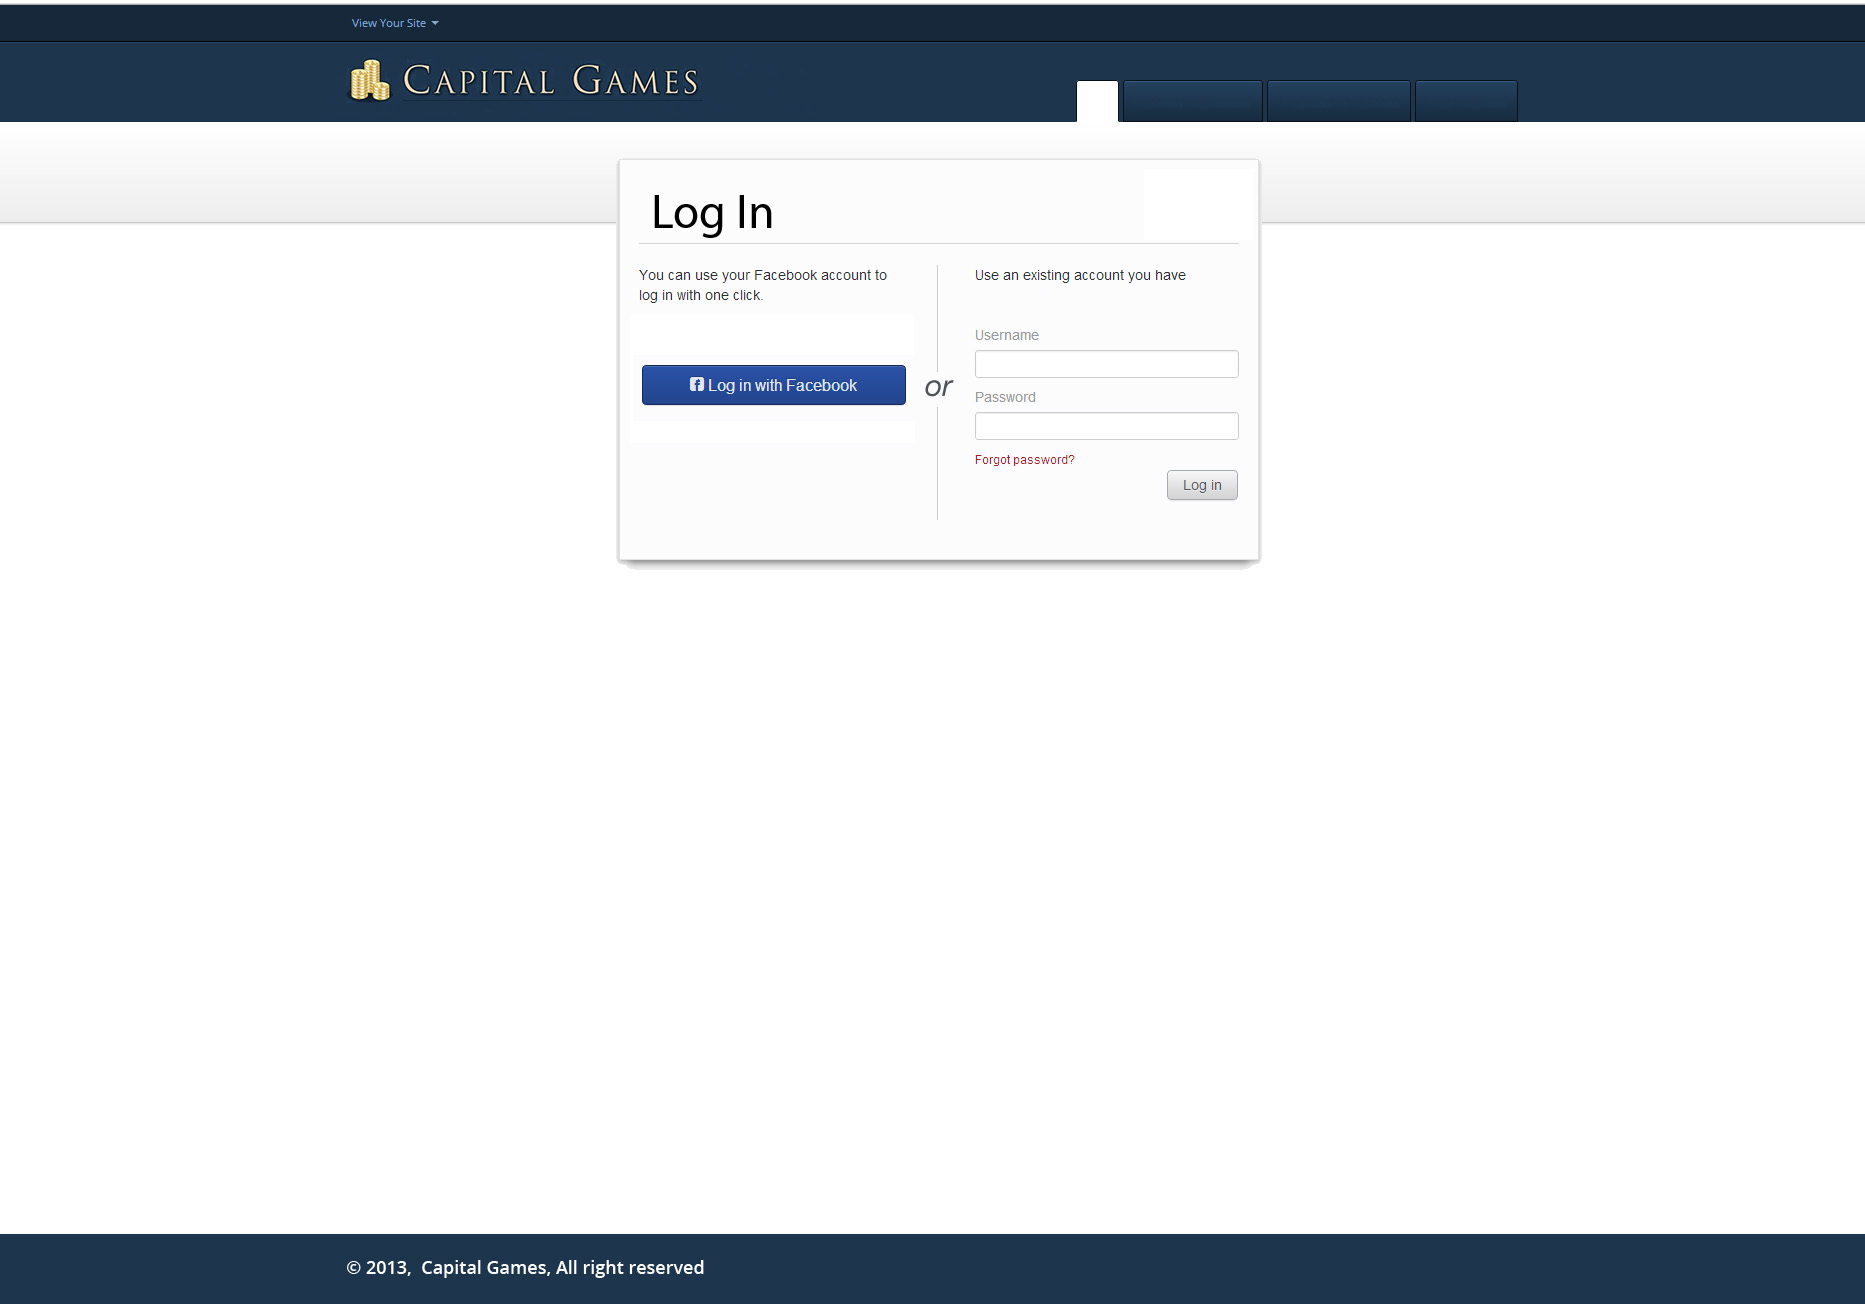
\includegraphics[width=5.5in]{./mockups/JPEG/Login.jpg}
\caption{Users would be able to login simply by clicking a login button on the top-right hand corner of the screen, which would take them to a prompt in which they can enter their username and password. This would only require one click and about 20 keystrokes from any page of the website. Users logged in to facebook may also take advantage of Facebook integration and instantly log in with 1 click.}
\end{figure}
}
%\vspace

\subection{Register}
{
\begin{figure}
\centering
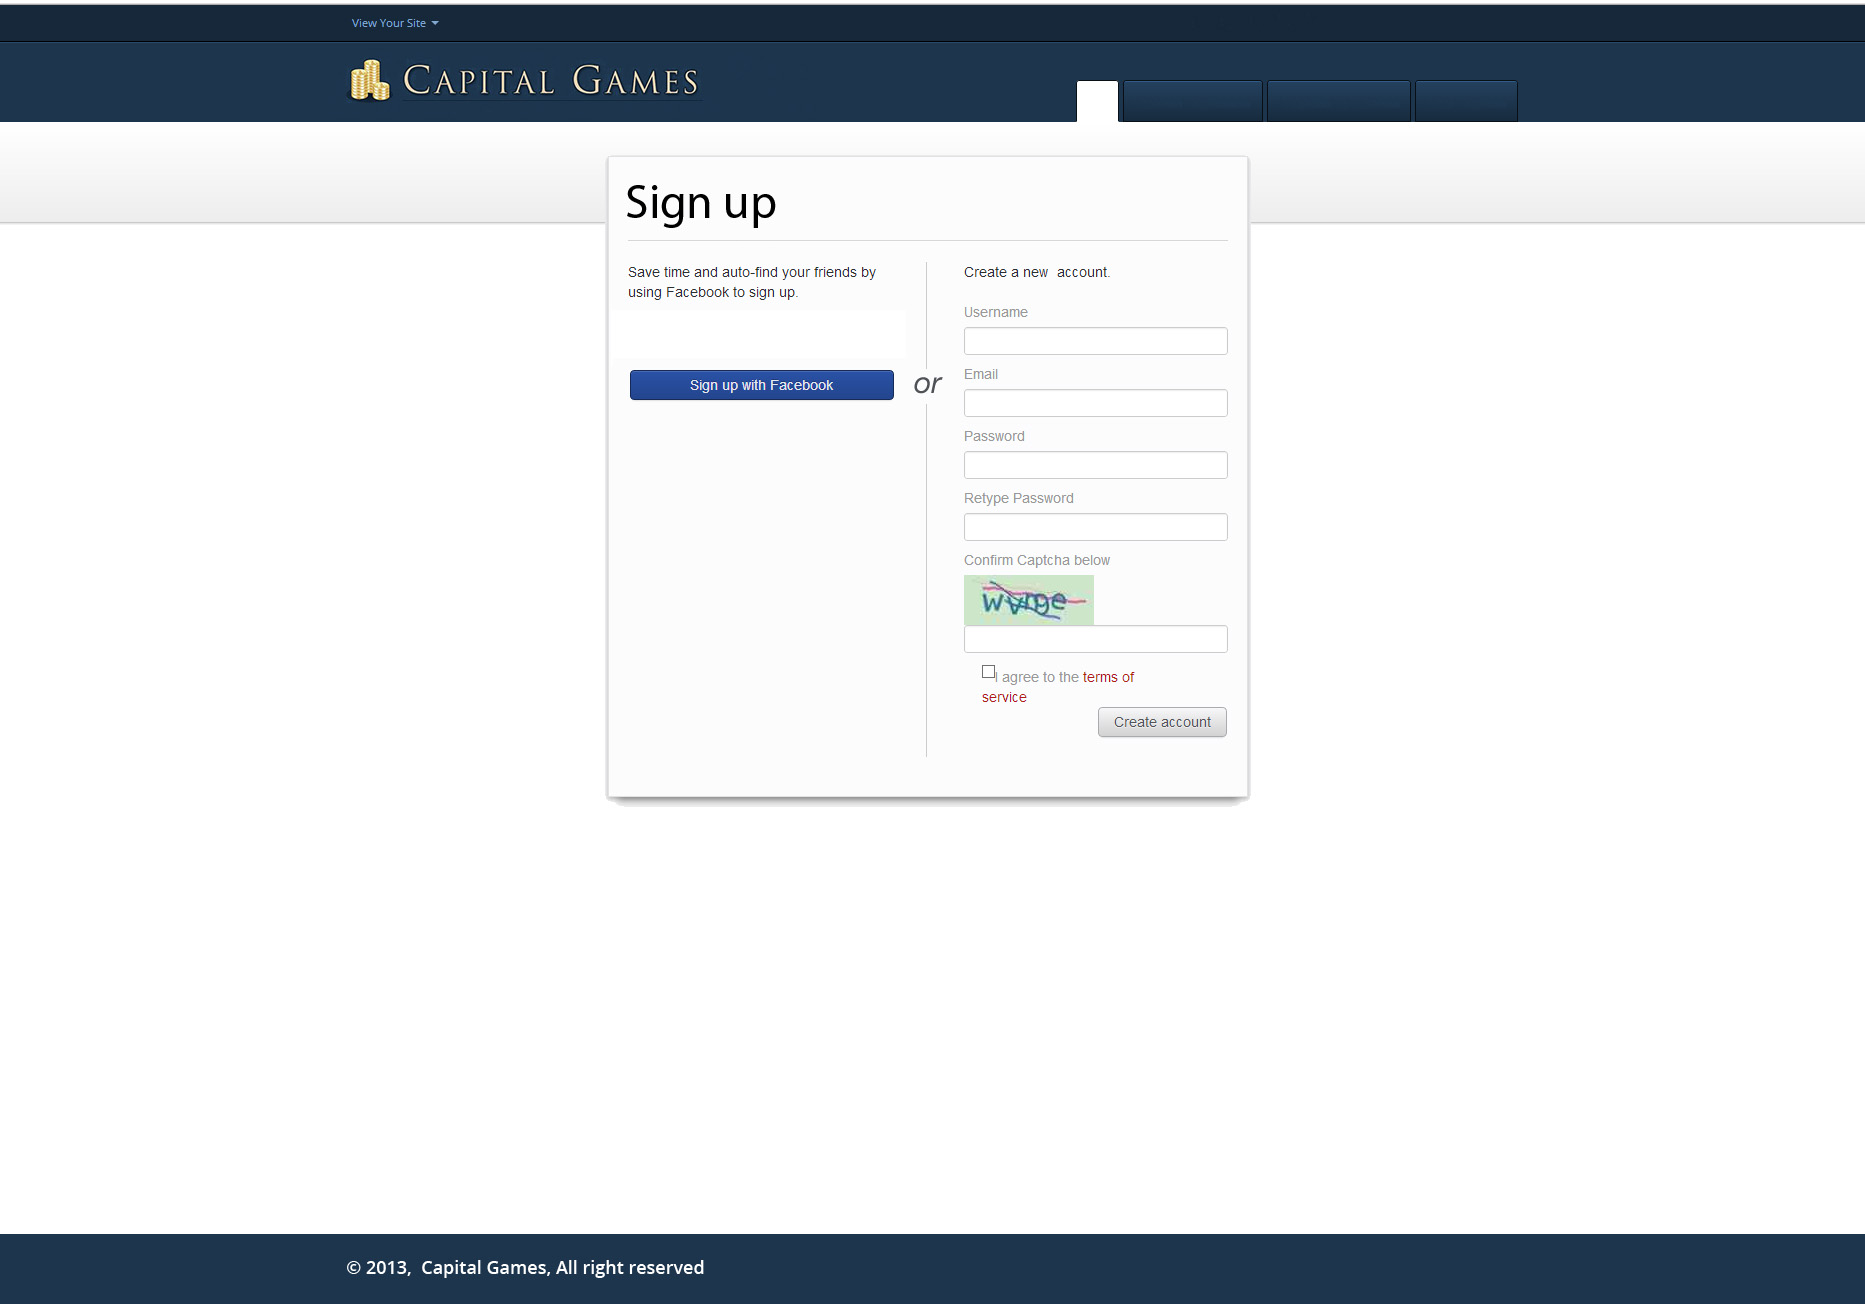
\includegraphics[width=5.5in]{./mockups/JPEG/Register.jpg}
\caption{Users who are not logged in will also have the ``Sign Up'' button available to them in the header that will enable them to register for Capital Games. This can be accomplished within 1 click and 50 keystrokes. A user logged in to facebook may also instantly register within 1 click.}
\end{figure}
}
%\vspace

\subsection{Portfolio}
{
\begin{figure}
\centering
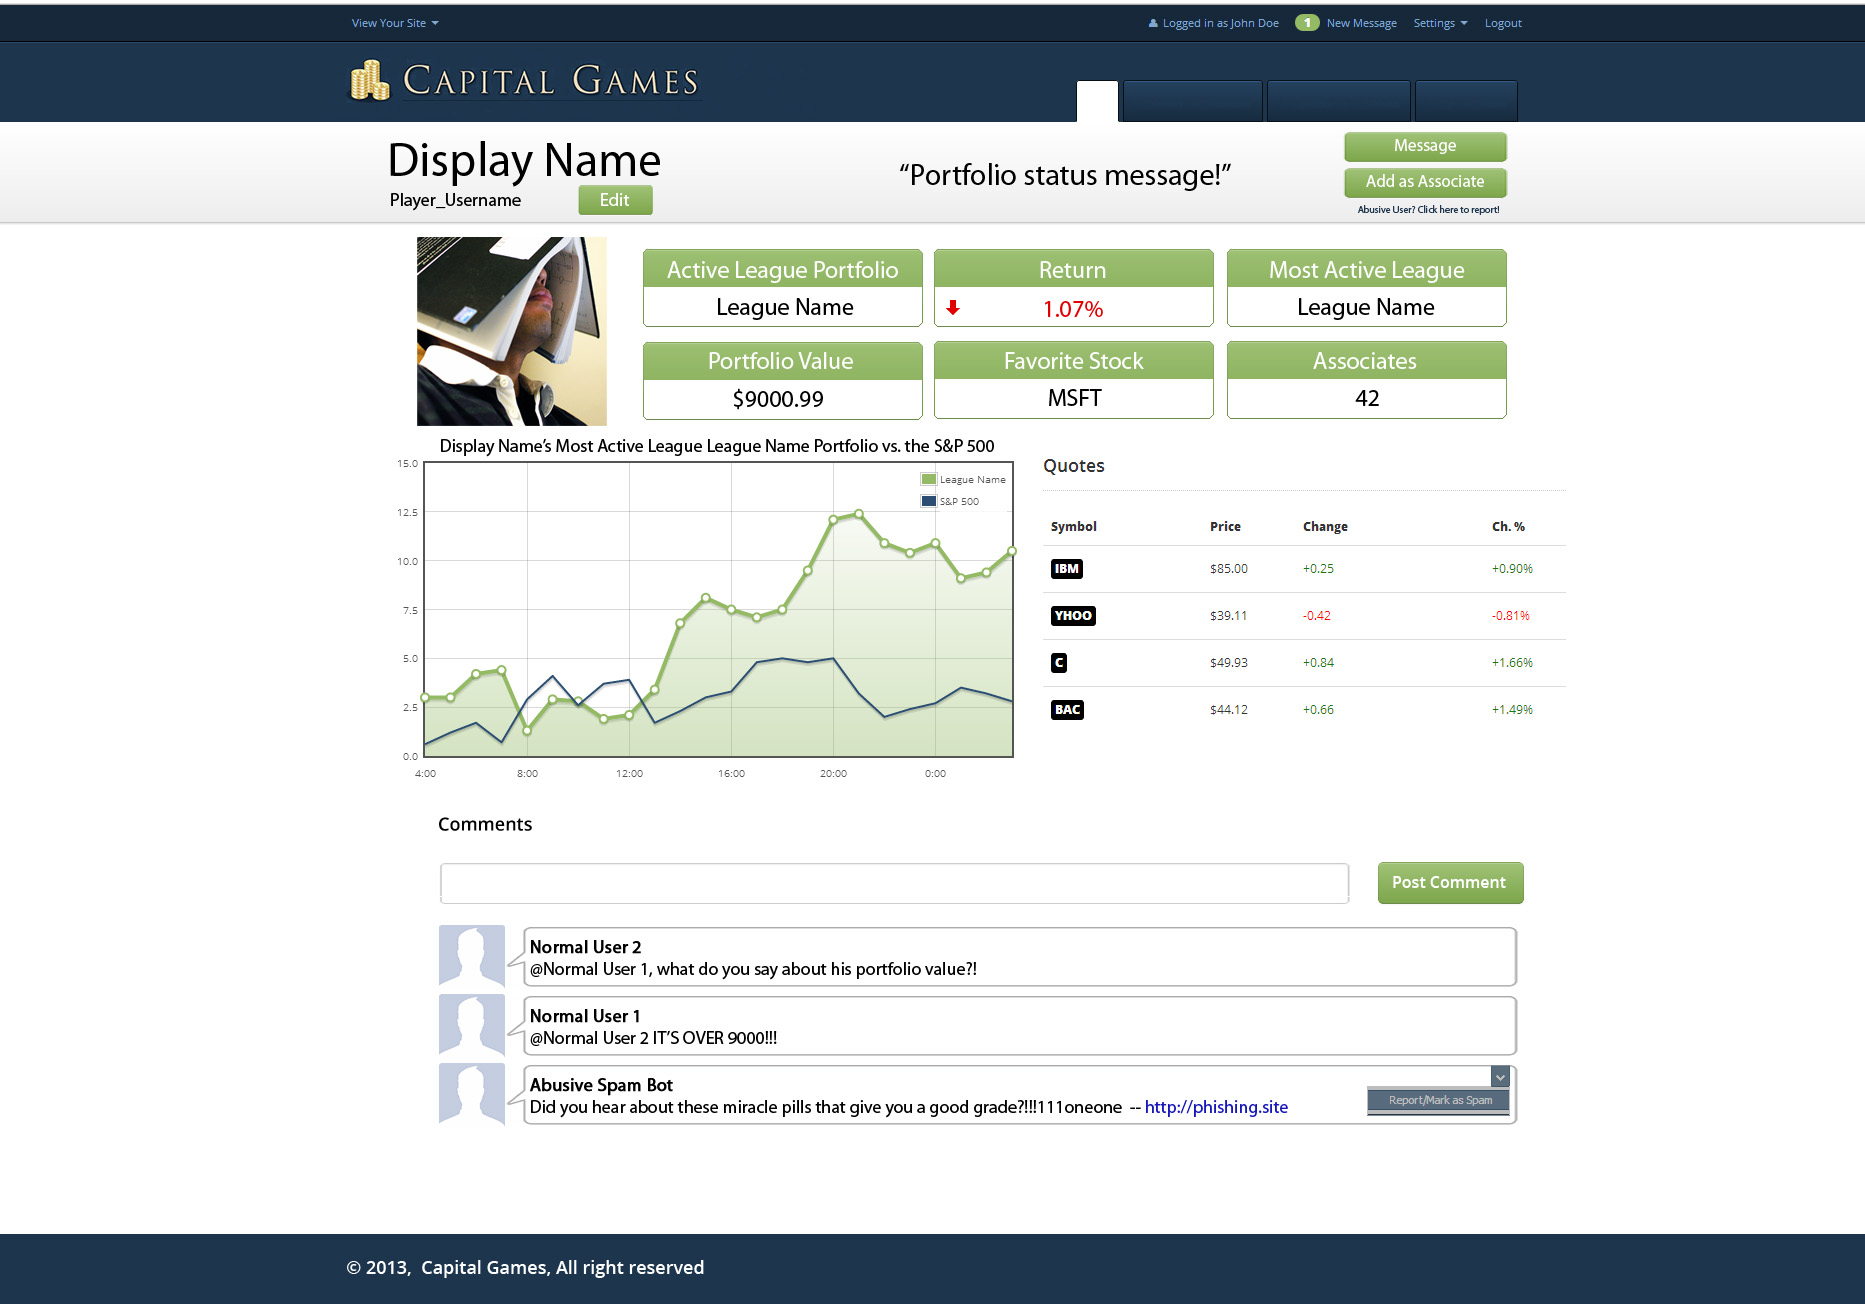
\includegraphics[width=5.5in]{./mockups/JPEG/Portfolio.jpg}
\caption{Users may access their Portfolio by clicking a menu tab in the top header of the website. This view enables them to conveniently see a summary of their return, active league, portfolio value, stock, and other data pertaining to their stock. They would be able to edit it in one click via the edit button. }
\end{figure}
}
%\vspace

\subsection{User Management}
{
\begin{figure}
\centering
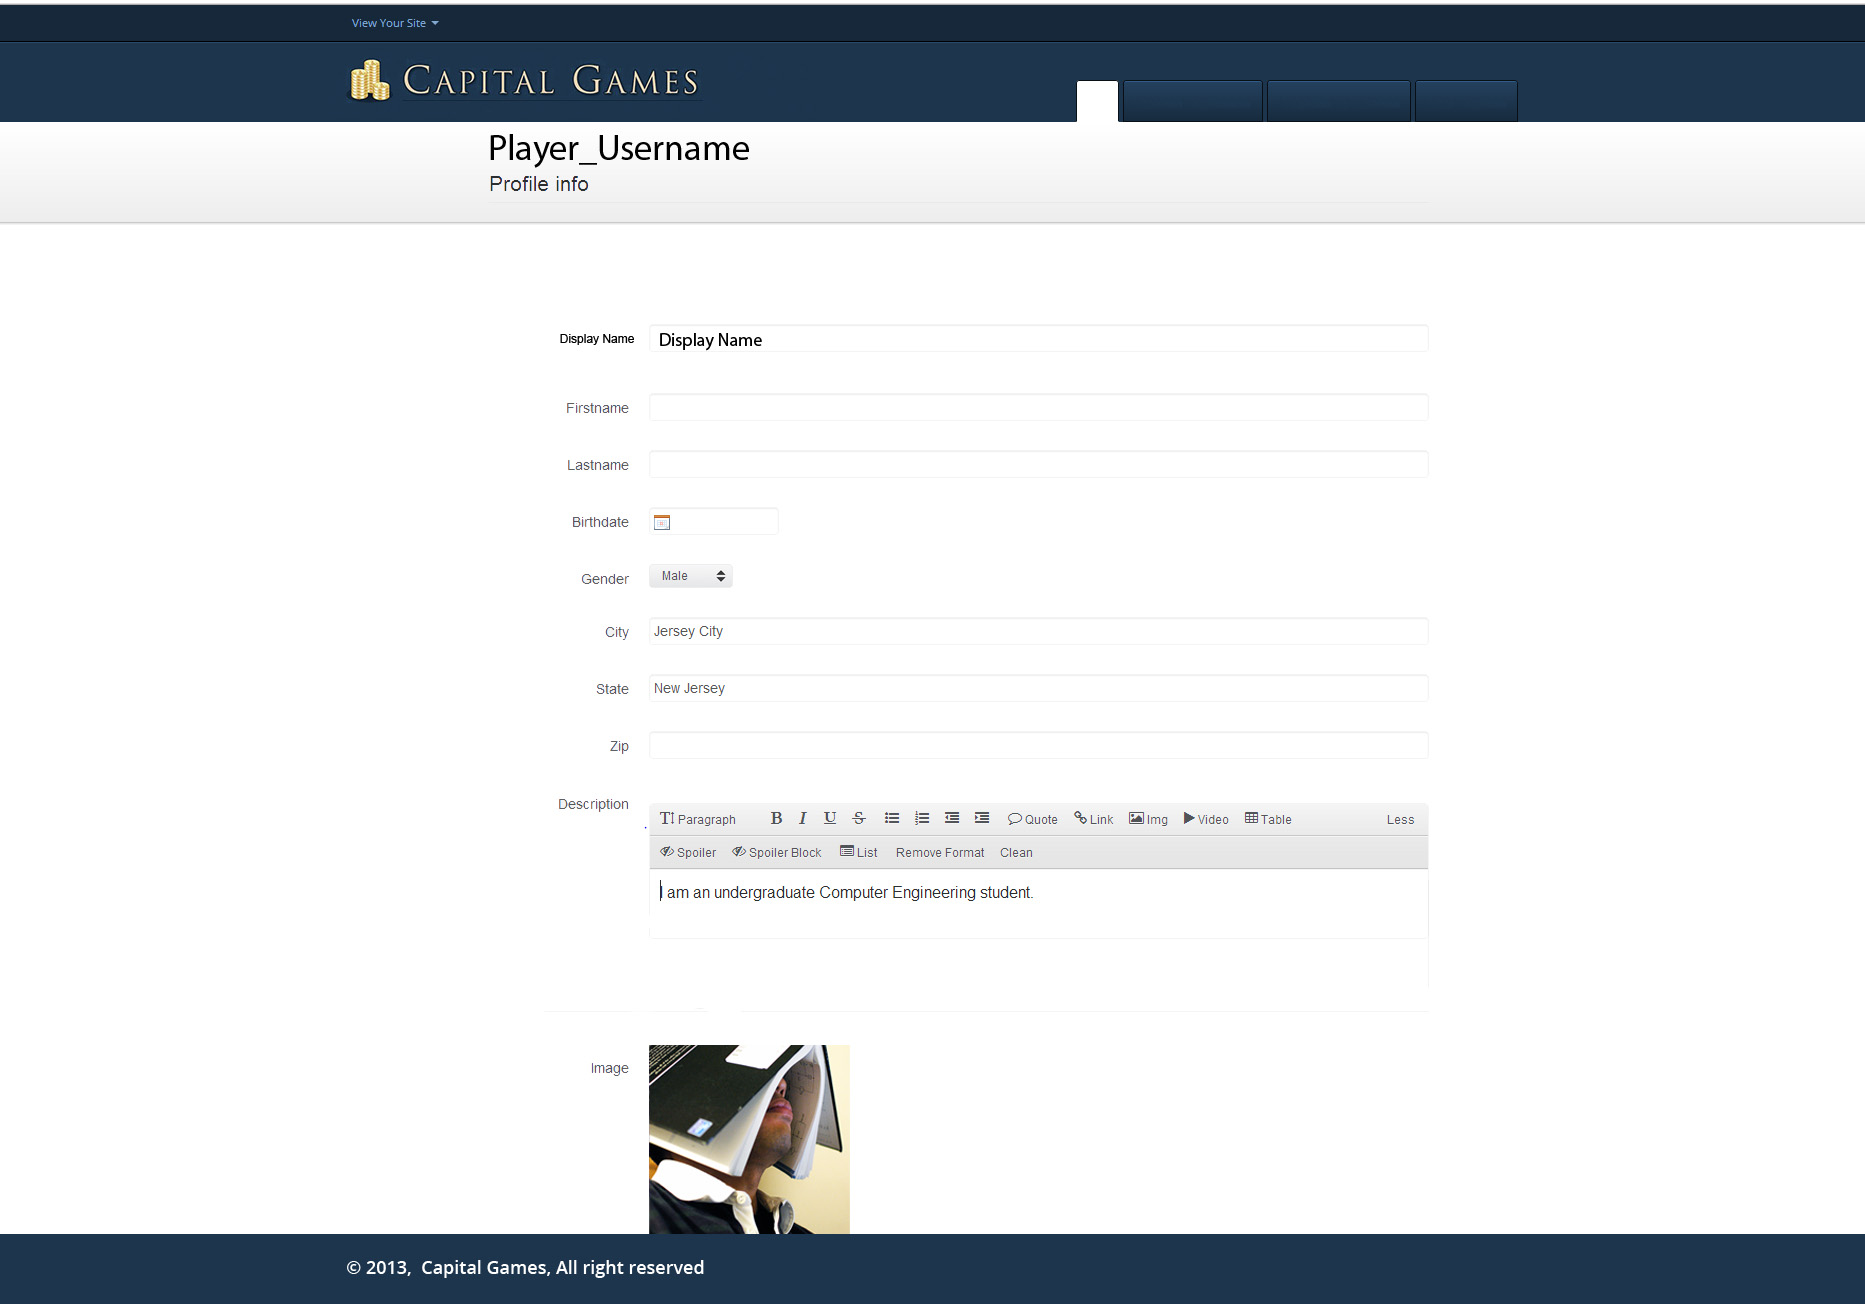
\includegraphics[width=5.5in]{./mockups/JPEG/ProfileManagement.jpg}
\caption{Upon clicking the ``Edit'' button on their portfolio page, users will also be able to manage profile items such as their display name, e-mail address, and other optional information they may choose to disclose, such as their name.}
\end{figure}
}
%\vspace

\subsection{Report}
{
\begin{figure}
\centering
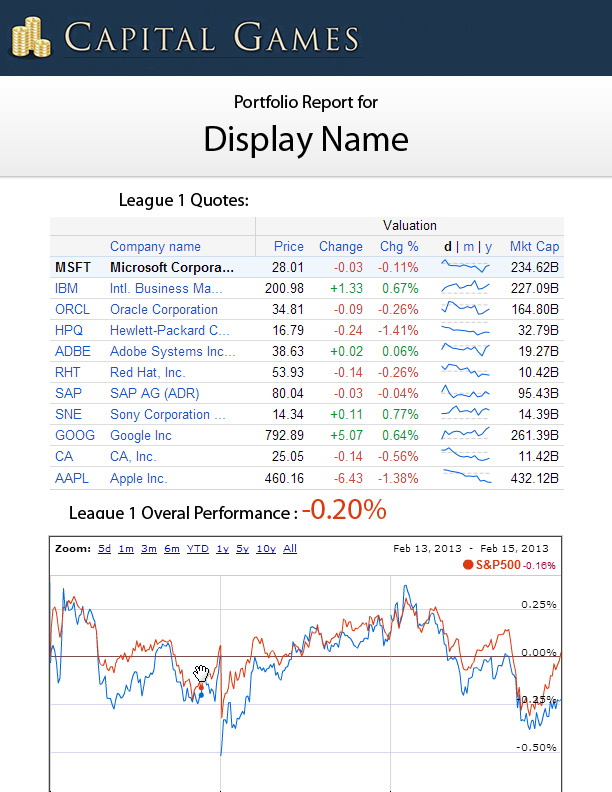
\includegraphics[width=5.5in]{./mockups/JPEG/Report.jpg}
\caption{Users may choose to view a summary report of a league portfolio, only requiring one click from the portfolio page which would sum to two clicks.}
\end{figure}
}
%\vspace

% This section contains lots of explanations
% of user effort and ease of access
% See Appendix A for examples to boost grade
\section{User Effort Estimation}